\documentclass[a4paper, 10pt]{article}
\usepackage[a4paper, total={6in, 10in}]{geometry}
\usepackage[printsolution=true]{exercises}
\usepackage{url}
\usepackage{float}
\usepackage{background, hyperref}
\usepackage{tcolorbox}
\usepackage[export]{adjustbox}
\usepackage{lastpage}
\usepackage{fancyhdr}
\usepackage{xcolor}
\usepackage[sfdefault]{cabin}
\usepackage{graphicx}
\usepackage{wrapfig}
\usepackage[T1]{fontenc}
\usepackage[backend=bibtex,style=authoryear,natbib=true, maxbibnames=9, maxcitenames=2]{biblatex}
\bibliography{howeetal18.bib}
\usepackage{todonotes}
%\bibliographystyle{besjournals}
\setlength\parindent{0pt}
\pagestyle{fancy}
\fancyhead[L,C,R]{}
\fancyfoot[L]{\small CTDS workshop, Univ. of St Andrews}
\fancyfoot[R]{\small Practical 5 - multipliers and density estimation}
\fancyfoot[C]{\small \thepage\ of \pageref{LastPage}}
\renewcommand{\headrulewidth}{0pt}
\renewcommand{\footrulewidth}{1pt}

\newif\iffirstpage
\firstpagetrue
\backgroundsetup{contents={%
 			\iffirstpage
				\includegraphics[width=\textwidth]{images/jaguar1.jpg}%
				\global\firstpagefalse
				\fi
			},
			scale=1,placement=top,opacity=0.6,position=current page.north, vshift=-1cm
}

\begin{document}
%% don't mess with blank lines here in the title.
\phantom{a}

\vspace{4.7cm}

{\Large Camera trap distance sampling workshop}

{\large 21-25 March 2022}

\begin{flushright}
\tiny{Source: \url{https://unsplash.com/@satyadeep_d}}
\end{flushright}

\ifsolutionthenelse{%
{\Large \color{blue}Solution \\}
{\color{blue}\rule{\linewidth}{0.5mm}}
}%
{%
}

Detection function modelling and selection of the most appropriate detection function model is now complete.  We will use the chosen model to estimate density from the camera trap data set of Maxwell's duikers.  However, before producing the density estimates, there are two adjustments to be made.

Those adjustments are called \emph{multipliers} and one multiplier is a known constant, while the second multiplier must be estimated and therefore contains uncertainty that must be propagated into our density estimates.

\section{Add more statistics to the \emph{Project Browser}}

With our interest now turned to the estimation of duiker density, we could expose more statistics in the \emph{Project Browser}.  However, given our focus will be upon a single analysis, we could omit this step.

\section{Field of view multiplier}

\begin{wrapfigure}{r}{0.35\textwidth}
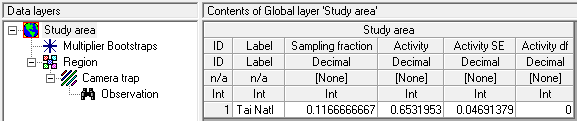
\includegraphics[width=0.33\textwidth]{images/global-data.png}
\caption{Multipliers in the global data layer. \label{fig:globaldata}}
\vspace{-25pt}
\end{wrapfigure}

Examine the data sheet (Fig. \ref{fig:globaldata}).  Looking only at the global layer, we see a field labelled \emph{Sampling fraction}. This is the proportion of a circle within the field of view of the cameras used in the duiker study.  It is a constant, measured without uncertainty.

\section{Temporal activity multiplier}

The other multiplier is the proportion of time animals are active while the cameras are in operation.  Cameras operate for 11.5 hours (0630 - 1800) during the field operation \citep{howeetal}.  Not all animals were active and capable of triggering the cameras during those hours of the day.

Methods developed by \citet{rowcliffe_2014} and implemented in \citet{activity_pkg} determine the proportion of time animals are active based upon the camera triggering events.  From Fig. \ref{fig:globaldata} , you can see this proportion is estimated to be roughly 0.65.  This is an estimate, based upon the sampling performed by the camera and modelled by \citet{activity_pkg}.  Consequently there is uncertainty in this quantity, reflected by the standard error reported in the global data layer of 0.047.

\subsection{Computation of temporal activity multiplier}

As noted above, the estimate of the temporal activity multiplier is derived from an R package \citet{activity_pkg}.  This is where the estimate of 0.65 and its standard error of 0.047 were derived.  

We will leave these values as they are for the moment, later in this practical we will use an interface to \citet{activity_pkg} for an alternative way to compute uncertainty in the temporal activity multiplier.  You will also want experience using the interface to \citet{activity_pkg} with your own data.


\section{Inclusion of multipliers in density estimates}

\begin{wrapfigure}{r}{0.35\textwidth}
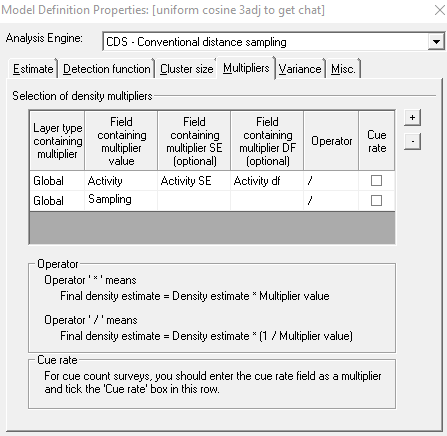
\includegraphics[width=0.33\textwidth]{images/multiplier-tab.png}
\caption{Multipliers in the global data layer. \label{fig:multtab}}
\vspace{-25pt}
\end{wrapfigure}
Just because multipliers have been supplied in the data sheet, they are not necessarily incorporated in the analyses.  We must check the \emph{Multipliers} tab associated with our analyses (Fig. \ref{fig:multtab}).  From this figure, note that both multipliers have been included in the analysis.

\section{Produce a density estimate with multipliers}

Now that all the set-up has been done, examine the analysis using your preferred model with both multipliers implemented to estimate duiker density and note the uncertainty in the estimate.


\section{Interface to \citet{activity_pkg} software}

The activity pattern analysis software \citep{activity_pkg} is an R package.  We have developed a way of using this software without the need to know the R language.  By opening a browser to this address


\url{https://lenthomas.shinyapps.io/Activity/}

%\begin{wrapfigure}{r}{0.35\textwidth}
\begin{figure}[H]
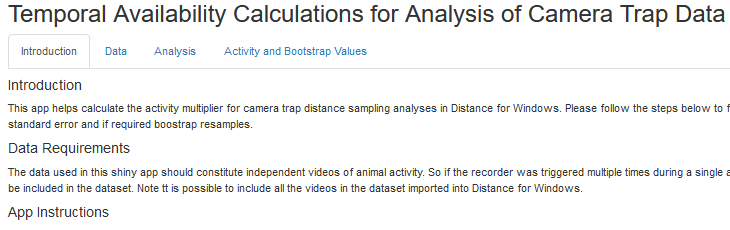
\includegraphics[width=\textwidth, frame]{images/shiny-tab1.png}
\caption{Opening tab of online application. \label{fig:sh1}}

\end{figure}
%\vspace{-25pt}
%\end{wrapfigure}
you will be able to upload your camera triggering data and analyse them to estimate the proportion of time animals are active.  Extensive instructions about the application are found when the application opens (Fig. \ref{fig:sh1}).

\subsection{Input data into Shiny}
%\begin{wrapfigure}{r}{0.35\textwidth}
\begin{figure}[H]
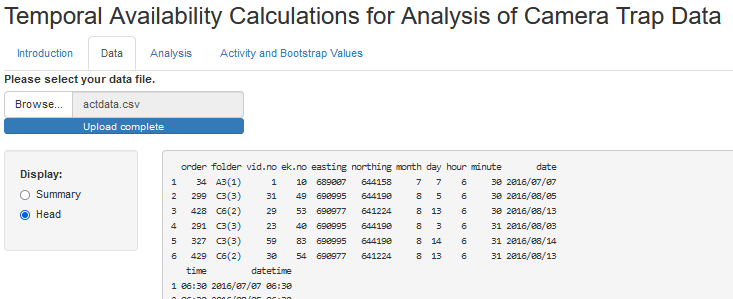
\includegraphics[width=\textwidth, frame]{images/shiny-tab2.png}
\caption{Data input tab of online application. \label{fig:sh2}}
%\vspace{-25pt}
\end{figure}
%\end{wrapfigure}

Upload a data file from your local computer to the cloud-based application (Fig. \ref{fig:sh2}).  The file can contain any number of fields as long as the time of camera triggerings are within the file.  For this practical, use the comma-delimited value file \textbf{\texttt{actdata.csv}} found in the Practical 5 folder of our Teams web site.

\subsection{Create bootstraps}
%\begin{wrapfigure}{r}{0.35\textwidth}
\begin{figure}[H]
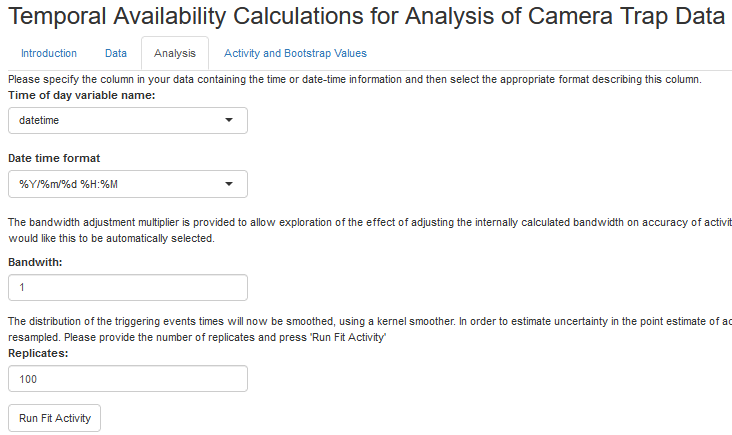
\includegraphics[width=\textwidth, frame]{images/shiny-tab3.png}
\caption{Temporal availability calculation tab of online application. \label{fig:sh3}}
\end{figure}
%\vspace{-25pt}
%\end{wrapfigure}

Uncertainty in the temporal availability multiplier is estimate by resampling the camera triggering times.  The smoothness of the kernel density model can be adjusted using the bandwidth argument (Fig. \ref{fig:sh3}).  Simulations by \citet{rowcliffe_2014} suggests best performance with bandwidth of \textbf{1.5}.  Further details regarding calculation of the temporal availability multiplier can be found in \citet{activity_pkg}.  Create \textbf{500} replicates in this step for later use.


\subsection{Adjust for camera hours of operation}

%\begin{wrapfigure}{r}{0.35\textwidth}
\begin{figure}[H]
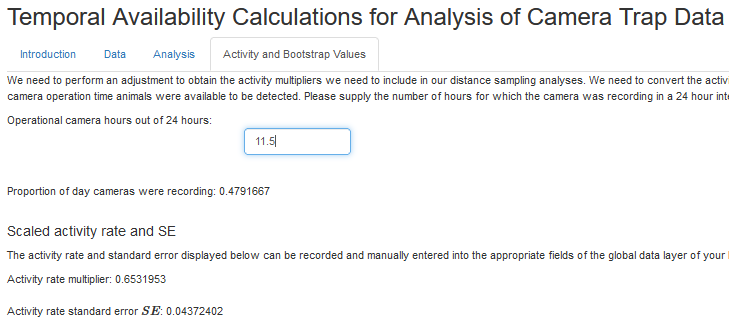
\includegraphics[width=\textwidth, frame]{images/shiny-tab4.png}
\caption{Camera hour adjustment tab, with download button (not shown) at the bottom of this tab of the app. \label{fig:sh4}}
\end{figure}
%\vspace{-25pt}
%\end{wrapfigure}

The temporal availability computations operate under the assumption that the cameras operate 24 hours per day.  If that is true for your study, no adjustment is necessary.  For the study described in \citet{howeetal}, cameras were operational for 11.5 hours per day.  This adjustment is implemented in Fig. \ref{fig:sh4}.  After adjustment, the bootstrap replicates created by \citet{activity_pkg} can be downloaded from the cloud-based app to your local computer.

\subsection{Download bootstraps and import into Distance for Windows}
\begin{wrapfigure}{r}{0.45\textwidth}
%\begin{figure}[H]
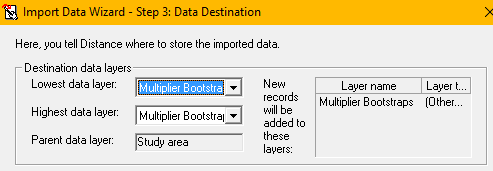
\includegraphics[width=0.45\textwidth, frame]{images/import-layer.png}
\caption{Specifying the data layer into which the bootstrap replicate file will be imported. \label{fig:i-layer}}
%\end{figure}
\vspace{-25pt}
\end{wrapfigure}


After downloading the file of bootstrap replicate estimates of the temporal availability multiplier, these replicates can be imported into Distance for Windows using the \emph{Import Data Wizard}.  Uncertainty in the density estimates can then include bootstrap estimates of temporal availability multiplier, rather than analytical estimates of multiplier uncertainty shown at the bottom of Fig. \ref{fig:sh4}.
\bigskip
Importing a file into Distance for Windows is described in the users guide for that software.  With the temporal availability multiplier, the file of bootstrap replicates is imported into the Multiplier Bootstrap layer (Fig. \ref{fig:i-layer}).

Both the layer and the field name must be specified before the input can take place (Fig. \ref{fig:i-file}).
\begin{wrapfigure}{l}{0.45\textwidth}
%\begin{figure}[H]
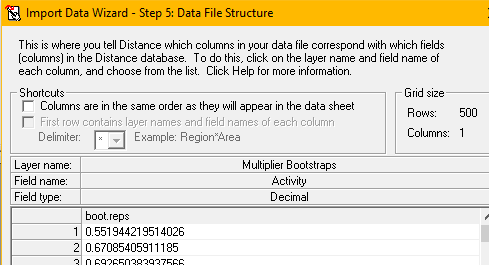
\includegraphics[width=0.45\textwidth, frame]{images/import-filestructure.png}
\caption{Associating the bootstrap replicate file with the proper field and data layer. \label{fig:i-file}}
%\end{figure}
\vspace{-25pt}
\end{wrapfigure}

Once the bootstrap replicates have been imported, they will not be used in the uncertainty of density estimates until Distance for Windows is instructed to use bootstrap rather than analytical means of estimating multiplier uncertainty.  This dialogue takes place in the Variance tab shown in Fig. \ref{fig:i-boot}.

\begin{wrapfigure}{l}{0.45\textwidth}
%\begin{figure}[H]
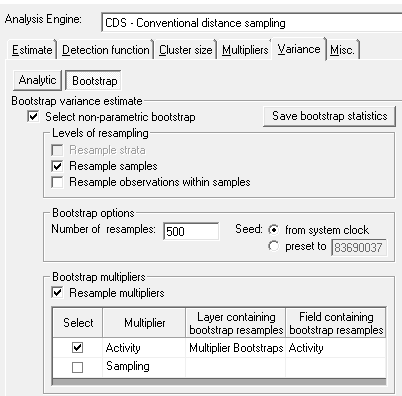
\includegraphics[width=0.45\textwidth, frame]{images/import-boot-activity.png}
\caption{Instructing Distance for Windows to resample the imported bootstrap replicates to estimate uncertainty in temporal availability multiplier. \label{fig:i-boot}}
%\end{figure}
\vspace{-25pt}
\end{wrapfigure}

\begin{wrapfigure}{r}{0.35\textwidth}
%\begin{figure}[H]
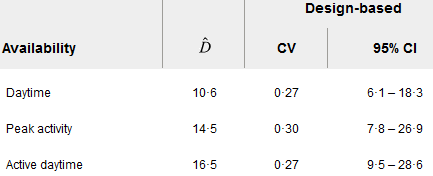
\includegraphics[width=0.33\textwidth]{images/density-table.png}
\caption{Density estimates from \citet{howeetal}.  Incorporating both multipliers would make your estimate comparable to that labelled \emph{Active daytime}. \label{fig:dentab}}
%\end{figure}
\vspace{-25pt}
\end{wrapfigure}
\vspace{.6in}

By selecting the non-parameteric bootstrap (topmost check box, Fig. \ref{fig:i-boot}), the camera stations will be resampled with replacement (second-top check box, Fig. \ref{fig:i-boot}) to refit the detection function and estimate the encounter rate variance.  The third and fourth check boxes of Fig. \ref{fig:i-boot} ensure that the replicate estimates of the activity multiplier are also used to compute uncertainty in the density estimate. Note the number of replicates requested here \textbf{must match} the number of bootstrap replicates created with the Shiny app.  If the last two check boxes of Fig. \ref{fig:i-boot} are not ticked, the activity multiplier will be assumed constant and uncertainty in the multiplier will not be propagated through to uncertainty in the density estimate.

\section{Questions about this analysis}


\begin{itemize}
	\item How does the estimate of density and its precision compare with the results presented in \citet{howeetal} (Fig. \ref{fig:dentab})?
\ifsolutionthenelse{%
	\begin{tcolorbox}[colback=green!5!white, colframe=green!60!black, title=Model selection choices]
	\citet{howeetal} used the hazard rate key function without adjustments as basis for inference. Because we used a different candidate model set (and enhanced the computation of the activity multiplier), our density estimate of 18.4 duikers $\cdot \textsf{hectare}^{-1}$ differs from the published estimate of 16.5 duikers $\cdot \textsf{hectare}^{-1}$.  The coefficients of variation for the two density estimates are very similar (0.28 in this analysis, 0.27 in the published study).
\end{tcolorbox}
}
{
}
	\item What is the consequence of using bootstrap estimates of uncertainty compared to analytical measures of uncertainty?
\ifsolutionthenelse{%
	\begin{tcolorbox}[colback=green!5!white, colframe=green!60!black, title=Differences in confidence interval bounds on $\hat{D}$]
		Confidence interval bounds widen from (10.4, 32.5) analytical to (8.4, 38.8) bootstrap. Your bootstrap confidence interval bounds will differ from these because of the stochasticity of the bootstrap.
		\end{tcolorbox}
}
{
}
\end{itemize}

\printbibliography

\end{document}